
\section{\floweroneleft OpenStreetMap with Hill Shade Layers}
\label{sec-1}

Although I was born in Madrid, Galicia (north of Spain) is a very
special region for me. More precisely, the Cedeira and Valdoviño
regions offer a wonderful combination of wild sea, secluded beaches,
and forests. I will show you a map of these marvelous places.

\subsection{Retrieving Data from OpenStreetMap}
\label{sec-1-1}
The first step is to acquire information from the OpenStreetMap
project. There are several packages to extract data from this service
but, while most of them only provide already rendered raster images,
the \texttt{osmar} package\footnote{Its webpage \url{http://osmar.r-forge.r-project.org/} proposes
two interesting demos.} \cite{Eugster.Schlesinger2010} enables the
use of the raw data with classes from the packages \texttt{sp} and \texttt{igraph}.

The \texttt{get\_osm} function retrieves a region defined by \texttt{corner\_bbox}
using the OSM API.

\index{Data!OpenStreetMap}
\index{Packages!osmar@\texttt{osmar}}
\index{osmsource_api@\texttt{osmsource\_api}}
\index{get_osm@\texttt{get\_osm}}

\lstset{language=R,numbers=none}
\begin{lstlisting}
library('osmar')

api <- osmsource_api()
ymax <- 43.7031
ymin <- 43.6181
xmax <- -8.0224
xmin <- -8.0808
box <- corner_bbox(xmin, ymin, xmax, ymax)
cedeira <- get_osm(box, source=api, full=TRUE)
\end{lstlisting}

The \texttt{cedeira} object includes three main components: nodes, ways and
relations. These components can be accessed with the functions \texttt{find},
\texttt{subset}, \texttt{way}, \texttt{node}, \texttt{relation}, and \texttt{tags}. Thus, the different
kinds of roads can be obtained using \texttt{way} and \texttt{tags} with the
appropiate tag.

\lstset{language=R,numbers=none}
\begin{lstlisting}
summary(cedeira$nodes)
\end{lstlisting}

\index{find@\texttt{find}}
\index{subset@\texttt{subset}}
\index{way@\texttt{way}}

\lstset{language=R,numbers=none}
\begin{lstlisting}
idxHighways <- find(cedeira, way(tags(k=='highway')))
highways <- subset(cedeira, way_ids=idxHighways)
idxStreets <- find(highways, way(tags(v=='residential')))
idxPrimary <- find(highways, way(tags(v=='primary')))
idxSecondary <- find(highways, way(tags(v=='secondary')))
idxTertiary <- find(highways, way(tags(v=='tertiary')))
idxOther <- find(highways,
		 way(tags(v=='unclassified' |
			  v=='footway' |
			  v=='steps')))
\end{lstlisting}

The result of \texttt{find} is the index of each element. The correspondent
spatial object is extracted with \texttt{find\_down} and \texttt{subset}, and can be
converted to a class defined by the \texttt{sp} package with \texttt{as\_sp}. The
following \texttt{spFromOSM} function encodes the procedure, and extracts the
\texttt{SpatialLines} object that represent each type of road.

\index{as_sp@\texttt{as\_sp}}
\index{find_down@\texttt{find\_down}}

\lstset{language=R,numbers=none}
\begin{lstlisting}
spFromOSM <- function(source, index, type='lines'){
  idx <- find_down(source, index)
  obj <- subset(source, ids=idx)
  objSP <- as_sp(obj, type)
  }

streets <- spFromOSM(cedeira, way(idxStreets))
primary <- spFromOSM(cedeira, way(idxPrimary))
secondary <- spFromOSM(cedeira, way(idxSecondary))
tertiary <- spFromOSM(cedeira, way(idxTertiary))
other <- spFromOSM(cedeira, way(idxOther))
\end{lstlisting}

A similar procedure can be applied to construct a \texttt{SpatialPoints}
object with the collection of places with name:

\index{match@\texttt{match}}

\lstset{language=R,numbers=none}
\begin{lstlisting}
idxPlaces <- find(cedeira, node(tags(k=='name')))
places <- spFromOSM(cedeira, node(idxPlaces), 'points')

nms <- subset(cedeira$nodes$tags, subset=(k=='name'), select=c('id', 'v'))
ord <- match(idxPlaces, nms$id)
nms <- nms[ord,]
places$name <- nms$v[ord]

## Cedeira town will be printed differently
idxCedeira <- which(nms$v=='Cedeira') ##Main town
cedeiraCoords <- coordinates(places[idxCedeira,])
places <- places[-idxCedeira,]
\end{lstlisting}
\subsection{Hill Shading}
\label{sec-1-2}
\index{Hill shading}

The second step is to produce layers to display the topography. A
suitable method is shaded relief or hill shading. This technique
simulates the cast shadow thrown from a light source upon a raised
relief map. The hill shade layer can be computed from the slope and
aspect layers derived from a Digital Elevation Model (DEM). This layer
will underlay the DEM raster, which will be printed using
semitransparency.

The DEM for this region is available at the Geonetwork-SECAD service
from the Universidad de Extremadura and can be read with \texttt{raster}:

\index{Packages!raster@\texttt{raster}}
\index{Packages!rasterVis@\texttt{rasterVis}}
\index{Data!Geonetwork}

\lstset{language=R,numbers=none}
\begin{lstlisting}
library(raster)
## Galicia DEM
## http://ide.unex.es/geonetwork/srv/es/main.search?any=MDE_Galicia
## http://ide.unex.es:8180/geonetwork/srv/es/resources.get?id=21&fname=dem_gal.7z&access=private

old <- tempdir()
download.file('http://ide.unex.es:8180/geonetwork/srv/es/resources.get?id=21&fname=dem_gal.7z&access=private', 'dem_gal.7z')
unzip('dem_gal.7z')
demGalicia <- raster('dem_gal.asc')
setwd(old)
\end{lstlisting}

The \texttt{slope} and \texttt{aspect} layers are computed with the \texttt{terrain}
function, and the hill shade layer is derived with these layers for a
fixed sun position. Previously, the useful region of the DEM raster
was extracted with the \texttt{crop} function:

\index{terrain@\texttt{terrain}}
\index{crop@\texttt{crop}}
\index{hillShade@\texttt{hillShade}}
\index{Hill shading}

\lstset{language=R,numbers=none}
\begin{lstlisting}
cedeiraSP <- as_sp(cedeira, 'points')
projCedeira <- projection(cedeiraSP)
##extCedeira <- bbox(cedeiraSP) 
## or summary(cedeira$nodes)$bbox
extCedeira <- extent(-8.15, -7.95, 43.6, 43.75)
demCedeira <- crop(demGalicia, extCedeira)
projection(demCedeira) <- projCedeira
demCedeira[demCedeira <= 0] <- NA

slope <- terrain(demCedeira, 'slope')
aspect <- terrain(demCedeira, 'aspect')
hsCedeira <- hillShade(slope=slope, aspect=aspect,
		       angle=20, direction=30)
\end{lstlisting}
\subsection{Overlaying Layers of Information}
\label{sec-1-3}
And finally, the third step is to display the different layers of
information in correct order (Figure \ref{fig:cedeiraOsmar}):

\begin{itemize}
\item The hill shade layer is created with the \texttt{levelplot} method for
  \texttt{Raster} objects defined in the \texttt{rasterVis} package. The
  \texttt{GrTheme} is modified to display the sea region with blue color.

\item The DEM raster is printed with terrain colors and
semitransparency over the hill shade layer.

\item The roads are displayed with an auxiliary function (\texttt{sp.road})
that produces a colored line over a thicker black line.

\item The places are represented with \texttt{sp.points} and labeled with
the \texttt{sp.pointLabel} method, a modification of the \texttt{pointLabel}
function for \texttt{base} graphics, both defined in the \texttt{maptools}
package. These functions use optimization routines to find good
locations for point labels without overlaps.
\end{itemize}

\index{Packages!maptools@\texttt{maptools}}  
\index{Packages!sp@\texttt{sp}}  
\index{Packages!latticeExtra@\texttt{latticeExtra}}  
\index{Packages!colorspace@\texttt{colorspace}}  
\index{sp.lines@\texttt{sp.lines}}
\index{sp.lines@\texttt{sp.points}}
\index{sp.lines@\texttt{sp.pointLabel}}

\lstset{language=R,numbers=none}
\begin{lstlisting}
library(maptools)
library(latticeExtra)
library(colorspace)
library(rasterVis)

##Auxiliary function to display the roads. A thicker black line in
##the background and a thinner one with an appropiate color.
sp.road <- function(line, lwd=5, blwd=7,
		    col='indianred1', bcol='black'){
  sp.lines(line, lwd=blwd, col=bcol)
  sp.lines(line, lwd=lwd, col=col)
}

## The background color of the panel is set to blue to represent the sea
hsTheme <- modifyList(GrTheme(), list(panel.background=list(col='skyblue3')))
## DEM with terrain colors and semitransparency
terrainTheme <- modifyList(rasterTheme(region=terrain_hcl(n=15)),
				list(regions=list(alpha=0.6)))
## Hill shade and DEM overlaid
levelplot(hsCedeira, maxpixels=ncell(hsCedeira),
	  par.settings=hsTheme, margin=FALSE, colorkey=FALSE) +
  levelplot(demCedeira, maxpixels=ncell(demCedeira),
	    par.settings=terrainTheme) +
  ## Roads and places
  layer({
    ## Street and roads
    sp.road(streets, lwd=1, blwd=2, col='white')
    sp.road(other, lwd=2, blwd=3, col='white')
    sp.road(tertiary, lwd=3, blwd=4, col='palegreen')
    sp.road(secondary, lwd=4, blwd=6, col='midnightblue')
    sp.road(primary, col='indianred1')
    ## Places except Cedeira town
    sp.points(places, pch=19, col='black', cex=0.4, alpha=0.8)
    sp.pointLabel(places, labels=places$name,
		      fontfamily = 'Palatino', 
		      cex=0.6, col='black')
    ## Cedeira town
    panel.points(cedeiraCoords, pch=18, col='black', cex=1)
    panel.text(cedeiraCoords, labels='Cedeira', pos=2, offset=1)
    })
\end{lstlisting}

\begin{figure}[htb]
\centering
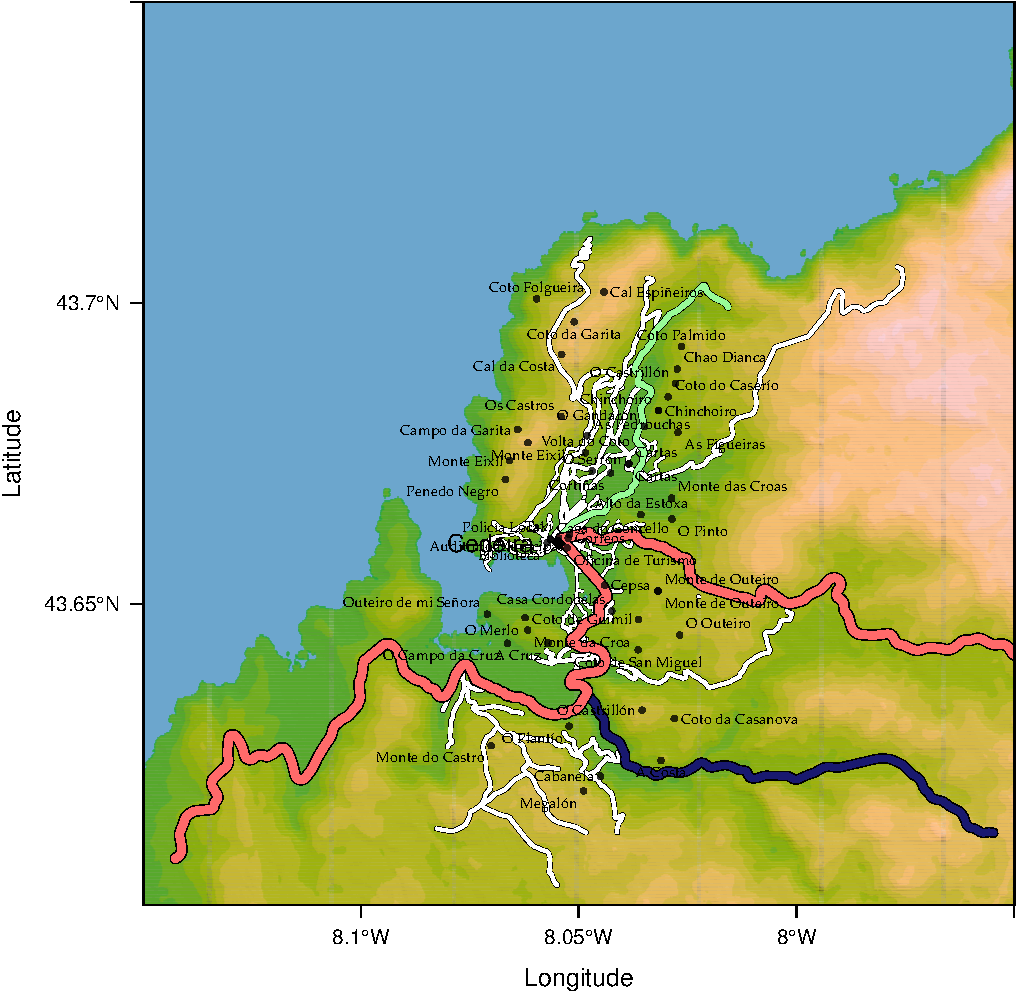
\includegraphics[width=.9\linewidth]{figs/cedeiraOsmar.pdf}
\caption{\label{fig:cedeiraOsmar}Main roads near Cedeira, Galicia. Local topography is displayed with the hill shading technique. Some places are highlighted.}
\end{figure}
